% !TEX TS-program = pdflatex
% !TEX encoding = UTF-8 Unicode

\documentclass{article}

\usepackage{kotex}
\usepackage[a4paper,left=35mm,right=35mm,top=40mm,bottom=40mm]{geometry}

\usepackage{graphicx}
\usepackage{listings}
\usepackage{color}

\definecolor{dkgreen}{rgb}{0,0.6,0}
\definecolor{gray}{rgb}{0.5,0.5,0.5}
\definecolor{mauve}{rgb}{0.58,0,0.82}

\lstset{frame=tb,
  language=Java,
  aboveskip=3mm,
  belowskip=3mm,
  showstringspaces=false,
  columns=flexible,
  basicstyle={\footnotesize},
  numbers=none,
  breaklines=true,
  breakatwhitespace=true,
  tabsize=3
}

\begin{document}

\title{프로그래밍 언어 HW3: YACC}
\author{B743014 양혜진}
\date{\today}
\maketitle

\section{YACC의 동작 방식}
YACC란 'Yet Another Compiler Compiler(또다른 컴파일러 컴파일러)'의 약자로, 
유닉스 시스템의 표준 파서 생성기이다. YACC는 프로그래밍 언어로 씌여진 원시 코드(source code)의
구문을 분석하여 구문 분석 트리(parse tree)를 자동적으로 생성하는 작업을 수행한다.

\vspace{3mm}
\noindent
YACC parser 는 입력값을 의미단위(token)로 나누는 어휘분석(Lexical Analysis) 프로그램인
Lex scanner 와 같이 구현하는 경우가 대부분이다. Lex 는 입력 문자열을 일차적으로 검색하여
Lex 기술 파일에 미리 정의된 정규표현식 규칙에 따라 토큰을 생성하여 반환한다. Yacc는 입력에 대한 토큰(token)
이 필요하면, Lex에서 제공하는 yylex() 함수를 호출하여 입력된 토큰들의 배열이 주어진 BNF 문법에 맞는지를
체크하면서 그 조건에 맞는 실행을 하게 된다.

\vspace{3mm}
\noindent
Lex와 YACC를 동시에 사용할 때는 YACC 기술 파일의 main() 함수에서 yyparse() 함수라는 YACC에서
만들어지는 구문분석기를 부르고, yyparse() 함수는 yylex()라는 Lex가 만들어 주는 해석기(lexer)를
이용해서 입력열에서 처리 단위의 토큰을 뽑아오게 된다.

\vspace{3mm}
\noindent
YACC 프로그램이 생성하는 파서는 본질적으로 stack 자료구조로 구현된 Finite State Machine
(유한 상태 기계)이다. State Machine 이란 여러 개의 상태(state)들을 어떤 조건에 따라 연결해
놓은 것으로, 이 중에서 유한한 갯수의 상태를 가진 것을 FSM(Finite State Machine) 이라고 한다.

\vspace{3mm}
\noindent
YACC 프로그램의 State Machine은 토큰을 계속 읽어서 사용자가 정의한 문법 규칙과 비교하며
구문 분석을 진행한다. 이때 읽어들인 토큰이 만족하는 문법(RHS)이 존재하지 않고 다른 토큰이 더 필요한 경우
토큰을 스택에 쌓아두는데, 이것을 스택에 적재(shift)힌다고 해서 shift 라고 부른다.
State Machine은 완전한 문법(RHS)이 스택에 올 때까지 token을 stack 에 반복적으로
적재(shift)하다가, 완전한 문법(RHS)에 해당하는 좌측(LHS)을 발견하면
스택에 있던 token을 꺼내고(pop) 문법의 좌측(LHS) symbol로 대치하는데,
이것을 감소(reduce)라고 한다.

\vspace{3mm}
\noindent
만약 하나의 token이 여러 개의 문법에 적용되어 한 번에 여러 개의 트리가 생성되는 모호한 문법의
경우 YACC는 다음 토큰을 하나 가져와서 문법을 비교하는데, 이 때 두 개 이상의 토큰을 가져와야
분석할 수 있는 문법이 있는 경우 YACC 파서가 제대로 구문 분석을 할 수 없으므로 주의해야 한다.

\begin{itemize}
	\item {\bf Compiler Compiler} : 컴파일러를 만들기 위한 컴파일러.
	구문 분석(parsing) 기능을 하는 프로그램과 같이 컴파일러 생성을 위한 프로그램을
	compiler-generator 또는 compiler-compiler라고 부른다.
	\item {\bf 파서(parser)} : 컴파일러의 일부로, 프로그래밍 언어로 씌여진 원시 코드(source code)를
	입력으로 받아들여 명령어 구문들의 구조를 알아내는 구문 분석(parsing)을 수행하는 프로그램이다.
	\item {\bf 구문 분석(parse)} : 주어진 문장이 정의된 문법 구조에 따라 정당하게 하나의 문장으로 사용될
	수 있는가를 확인하는 작업. 컴퓨터 분야에서는 컴파일러에 의하여 원시 코드(source code)를 기계어로 번역할
	때 낱말 분석(lexical analysis) 결과로 만들어진 토큰들을 문법에 따라 분석하는 파싱(parsing) 작업을
	수행하여 파싱 트리를 구성하는 작업을 지칭한다.
\end{itemize}

\section{YACC의 사용 방법}
YACC는 BNF(Backus Naur Form) 형식의 규칙 항목들로부터 parser 를 만들어낸다.
YACC 의 문법은 BNF 를 간단하게 만든 버전이다. YACC 는 Lex 와 비슷한 구조를 가지고 있다.
YACC 의 입력은 정의절, 규칙절, 서브루틴절 세 가지로 구성되어 있다. 이 중에서 정의절은
C 선언 부분과 YACC 선언 부분으로 나눌 수 있다.

\begin{lstlisting}
		%{
		정의절 - C 선언 부분(C Definition Section)
		%}
		정의절 - YACC 선언 부분(YACC Definition Section)
		%%
		규칙절 (Rules Section)
		%%
		사용자 서브루틴절(User Subroutines)
\end{lstlisting}

\begin{itemize}
	\item {\bf 정의절 - C 선언 부분(C Definition Section)} : 헤더파일을 include 하거나,
	규칙절이나 사용자 서브루틴절에서 사용할 변수나 함수의 원형(prototype)을 선언한다.
	\item {\bf 정의절 - YACC 선언 부분(YACC Definition Section)} : 문법 부분에서 사용하는
	토큰, 결합법칙, 변수나 토큰들의 타입 등을 선언한다. 이렇게 규칙절에 작성된 내용은
	yyparse()라는 구문 분석기 함수를 가진 y.tab.c라는 C 언어 파일에 복사된다.
	\item {\bf 규칙절(Rules Section)} : YACC가 인식할 BNF 형태의 문법과 그에 따라 취할
	C 언어로 된 행동을 정의한다. 각 rule은 "LHS: RHS;"와 같은 형식으로 이루어진다. LHS는
	left-hand symbol의 약자로, ':'의 왼쪽에 오는 nonterminal 기호를 말하며, RHS는
	right-hand symbol의 약자로, ':'의 오른쪽에 오는 기호를 말한다. 각 rule의 끝은 ';'으로
	표시하고, 문법에 따라 취할 행동은 '{'와 '}' 사이에 작성한다.
	\item {\bf 사용자 서브루틴절(User Subroutines)} : 사용자가 만들어서 사용해야 할 함수를 정의한다.
	대표적으로 yyerror()과 같이 yyparse() 에서 파싱 에러가 발생했을 때 호출되는 함수를 정의할 수 있다.
	또한, 규칙절의 C 선언 부분에 정의 했던 함수의 선언을 정의한다.
\end{itemize}

\newpage

\section{hw3.l}

\begin{itemize}
	\item 파일명 : hw3.l
	\item 내용 : ANSI C Lex Grammar를 바탕으로 입력값을 token으로 나누어 반환한다.
\end{itemize}

\subsection{hw3.l 소스 코드}
\begin{lstlisting}
		%{
		#include <stdio.h>
		#include "y.tab.h"
		%}
		
		D			[0-9]
		L			[a-zA-Z_]
		H			[a-fA-F0-9]
		E			[Ee][+-]?{D}+
		FS			(f|F|l|L)
		IS			(u|U|l|L)*
		%%
		"//"(.*)\n 					{;}
		"/*"([^\*]|(\*+[^\/]))*"*/" {;}
		"auto"			{ return(AUTO); }
		"break"			{ return(BREAK); }
		"case"			{ return(CASE); }
		"char"			{ yylval.type = 3; return(CHAR); }
		"const"			{ return(CONST); }
		"continue"		{ return(CONTINUE); }
		"default"		{ return(DEFAULT); }
		"define"		{ return(DEFINE); }
		"do"			{ return(DO); }
		"double"		{ return(DOUBLE); }
		"enum"			{ return(ENUM); }
		"extern"		{ return(EXTERN); }
		"float"			{ return(FLOAT); }
		"for"			{ return(FOR); }
		"goto"			{ return(GOTO); }
		"if"			{ return(IF); }
		"include"		{ return(INCLUDE); }
		"int"			{ yylval.type = 2; return(INT); }
		"long"			{ return(LONG); }
		"register"		{ return(REGISTER); }
		"return"		{ return(RETURN); }
		"short"			{ return(SHORT); }
		"signed"		{ return(SIGNED); }
		"sizeof"		{ return(SIZEOF); }
		"static"		{ return(STATIC); }
		"struct"		{ return(STRUCT); }
		"switch"		{ return(SWITCH); }
		"typedef"		{ return(TYPEDEF); }
		"union"			{ return(UNION); }
		"unsigned"		{ return(UNSIGNED); }
		"void"			{ return(VOID); }
		"volatile"		{ return(VOLATILE); }
		"while"			{ return(WHILE); }
		
		{L}({L}|{D})*		{ return(IDENTIFIER); }
		
		{L}+"."h	{ return(HEADER); }
		
		0[xX]{H}+{IS}?		{ return(CONSTANT); }
		0{D}+{IS}?		{ return(CONSTANT); }
		{D}+{IS}?		{ return(CONSTANT); }
		L?'(\\.|[^\\'])+'	{ return(CONSTANT); }
		
		{D}+{E}{FS}?		{ return(CONSTANT); }
		{D}*"."{D}+({E})?{FS}?	{ return(CONSTANT); }
		{D}+"."{D}*({E})?{FS}?	{ return(CONSTANT); }
		
		L?\"(\\.|[^\\"])*\"	{ return(STRING_LITERAL); }
		
		"..."			{ return(ELLIPSIS); }
		">>="			{ return(RIGHT_ASSIGN); }
		"<<="			{ return(LEFT_ASSIGN); }
		"+="			{ return(ADD_ASSIGN); }
		"-="			{ return(SUB_ASSIGN); }
		"*="			{ return(MUL_ASSIGN); }
		"/="			{ return(DIV_ASSIGN); }
		"%="			{ return(MOD_ASSIGN); }
		"&="			{ return(AND_ASSIGN); }
		"^="			{ return(XOR_ASSIGN); }
		"|="			{ return(OR_ASSIGN); }
		">>"			{ return(RIGHT_OP); }
		"<<"			{ return(LEFT_OP); }
		"++"			{ return(INC_OP); }
		"--"			{ return(DEC_OP); }
		"->"			{ return(PTR_OP); }
		"&&"			{ return(AND_OP); }
		"||"			{ return(OR_OP); }
		"<="			{ return(LE_OP); }
		">="			{ return(GE_OP); }
		"=="			{ return(EQ_OP); }
		"!="			{ return(NE_OP); }
		";"			{ return(';'); }
		("{"|"<%")		{ return('{'); }
		("}"|"%>")		{ return('}'); }
		","			{ return(','); }
		":"			{ return(':'); }
		"="			{ return('='); }
		"("			{ return('('); }
		")"			{ return(')'); }
		("["|"<:")		{ return('['); }
		("]"|":>")		{ return(']'); }
		"."			{ return('.'); }
		"&"			{ return('&'); }
		"!"			{ return('!'); }
		"~"			{ return('~'); }
		"-"			{ return('-'); }
		"+"			{ return('+'); }
		"*"			{ return('*'); }
		"/"			{ return('/'); }
		"%"			{ return('%'); }
		"<"			{ return('<'); }
		">"			{ return('>'); }
		"^"			{ return('^'); }
		"|"			{ return('|'); }
		"?"			{ return('?'); }
		"#"			{ return('#'); }
		
		[ \t\v\n\f.]		{;}
		
		%%
		
		int yywrap(void){
			return 1;
		}
\end{lstlisting}

\newpage

\subsection{hw3.l 코드 분석}
\begin{itemize}
	\item 정의절(Definitions Section)	
	\begin{itemize}
		\item {\bf 정의절 : C 선언 부분}
		\begin{lstlisting}
		%{
		#include <stdio.h>
		#include "y.tab.h"
		%}
		\end{lstlisting}
		입출력을 위해 stdio.h 헤더파일을 인클루드 했다.
		또한 lex 프로그램이 yacc 에서 정의한 토큰 값을 활용하기 위해 y.tab.h를 인클루드해야 한다.
		\item {\bf 추가적인 매크로 정의절}
		\begin{lstlisting}
		D			[0-9]
		L			[a-zA-Z_]
		H			[a-fA-F0-9]
		E			[Ee][+-]?{D}+
		FS			(f|F|l|L)
		IS			(u|U|l|L)*
		\end{lstlisting}
		규칙절에서 정규표현식의 패턴을 단순화하기 위해 사용할 변수를 선언했다.
		D는 숫자이고, L은 문자이다. E는 과학적 표기법 정규표현식을 단순화한 것이다.
	\end{itemize}

	\item 규칙절(Rules Section)	
	\begin{itemize}
		\item {\bf 규칙절 : 예약어 처리}
		\begin{lstlisting}
		"auto"			{ return(AUTO); }
		"break"			{ return(BREAK); }
		"case"			{ return(CASE); }
		"char"			{ yylval.type = 3; return(CHAR); }
		"const"			{ return(CONST); }
		"continue"		{ return(CONTINUE); }
		"default"		{ return(DEFAULT); }
		"define"		{ return(DEFINE); }
		"do"			{ return(DO); }
		"double"		{ return(DOUBLE); }
		"enum"			{ return(ENUM); }
		"extern"		{ return(EXTERN); }
		"float"			{ return(FLOAT); }
		"for"			{ return(FOR); }
		"goto"			{ return(GOTO); }
		"if"			{ return(IF); }
		"include"		{ return(INCLUDE); }
		"int"			{ yylval.type = 2; return(INT); }
		"long"			{ return(LONG); }
		"register"		{ return(REGISTER); }
		"return"		{ return(RETURN); }
		"short"			{ return(SHORT); }
		"signed"		{ return(SIGNED); }
		"sizeof"		{ return(SIZEOF); }
		"static"		{ return(STATIC); }
		"struct"		{ return(STRUCT); }
		"switch"		{ return(SWITCH); }
		"typedef"		{ return(TYPEDEF); }
		"union"			{ return(UNION); }
		"unsigned"		{ return(UNSIGNED); }
		"void"			{ return(VOID); }
		"volatile"		{ return(VOLATILE); }
		"while"			{ return(WHILE); }
		\end{lstlisting}
		예약어 auto, break, case, char, const, continue, default, define, do, double,
		enum, extern, float, for, goto, if, include, int, long, register, short, signed,
		sizeof, static, struct, switch, typedef, union, unsigned, void, volatile, while
		을 발견할 경우, 해당 예약어와 동일한 이름의 토큰을 반환하도록 정의했다. 다만, int 와 char 의 경우
		토큰의 값(value)를 리턴하여 Yacc 프로그램에서 yyval 로 사용할 수 있도록 했다.
		\item {\bf 규칙절 : IDENTIFIER}
		\begin{lstlisting}
		{L}({L}|{D})*		{ return(IDENTIFIER); }
		\end{lstlisting}
		위에서 정의한 예약어 이외의 단어는 모두 IDENTIFIER 토큰을 반환한다.

		\item {\bf 규칙절 : HEADER}
		\begin{lstlisting}
		{L}+"."h	{ return(HEADER); }
		\end{lstlisting}
		만약 .h 로 끝나는 단어가 있다면 헤더 파일의 이름이므로 HEADER 토큰을 반환한다.

		\item {\bf 규칙절 : CONSTANT}
		\begin{lstlisting}
		0[xX]{H}+{IS}?		{ return(CONSTANT); }
		0{D}+{IS}?		{ return(CONSTANT); }
		{D}+{IS}?		{ return(CONSTANT); }
		L?'(\\.|[^\\'])+'	{ return(CONSTANT); }
		
		{D}+{E}{FS}?		{ return(CONSTANT); }
		{D}*"."{D}+({E})?{FS}?	{ return(CONSTANT); }
		{D}+"."{D}*({E})?{FS}?	{ return(CONSTANT); }
		\end{lstlisting}
		숫자의 경우 10진수 뿐만 아니라 16진수, 8진수도 파악하여 CONSTANT 토큰을 반환한다.

		\item {\bf 규칙절 : STRING\_LITERAL}
		\begin{lstlisting}
		L?\"(\\.|[^\\"])*\"	{ return(STRING_LITERAL); }
		\end{lstlisting}
		큰 따옴표안에 있는 문자열은 문자열 리터럴 토큰을 반환한다.

		\item {\bf 규칙절 : ellipsis, assign, binary operator}
		\begin{lstlisting}
		"..."			{ return(ELLIPSIS); }
		">>="			{ return(RIGHT_ASSIGN); }
		"<<="			{ return(LEFT_ASSIGN); }
		"+="			{ return(ADD_ASSIGN); }
		"-="			{ return(SUB_ASSIGN); }
		"*="			{ return(MUL_ASSIGN); }
		"/="			{ return(DIV_ASSIGN); }
		"%="			{ return(MOD_ASSIGN); }
		"&="			{ return(AND_ASSIGN); }
		"^="			{ return(XOR_ASSIGN); }
		"|="			{ return(OR_ASSIGN); }
		">>"			{ return(RIGHT_OP); }
		"<<"			{ return(LEFT_OP); }
		"++"			{ return(INC_OP); }
		"--"			{ return(DEC_OP); }
		"->"			{ return(PTR_OP); }
		"&&"			{ return(AND_OP); }
		"||"			{ return(OR_OP); }
		"<="			{ return(LE_OP); }
		">="			{ return(GE_OP); }
		"=="			{ return(EQ_OP); }
		"!="			{ return(NE_OP); }
		\end{lstlisting}
		ellipsis 나 배정문 또는 이항 연산자의 경우 각각에 맞는 토큰을 반환한다.

		\item {\bf 규칙절 : unary operator}
		\begin{lstlisting}
		";"			{ return(';'); }
		("{"|"<%")		{ return('{'); }
		("}"|"%>")		{ return('}'); }
		","			{ return(','); }
		":"			{ return(':'); }
		"="			{ return('='); }
		"("			{ return('('); }
		")"			{ return(')'); }
		("["|"<:")		{ return('['); }
		("]"|":>")		{ return(']'); }
		"."			{ return('.'); }
		"&"			{ return('&'); }
		"!"			{ return('!'); }
		"~"			{ return('~'); }
		"-"			{ return('-'); }
		"+"			{ return('+'); }
		"*"			{ return('*'); }
		"/"			{ return('/'); }
		"%"			{ return('%'); }
		"<"			{ return('<'); }
		">"			{ return('>'); }
		"^"			{ return('^'); }
		"|"			{ return('|'); }
		"?"			{ return('?'); }
		"#"			{ return('#'); }
		\end{lstlisting}
		단항 연산자의 경우 자기 자신을 토큰으로 반환한다.

		\item {\bf 규칙절 : 공백}
		\begin{lstlisting}
		[ \t\v\n\f.]		{;}
		\end{lstlisting}
		공백 또는 위해서 작성한 규칙 이외의 문자열(.)은 무시한다.
	\end{itemize}

	\item 사용자 서브루틴절(User Subroutines Section)	
		\begin{lstlisting}
			int yywrap(void){
				return 1;
			}
		\end{lstlisting}
		Lex 와 Yacc 를 함께 사용하는 경우 Lex 파일 서브루틴절에서는 main()함수가 필요하지 않다.
		그러나 입력의 끝네 호출되는 yywrap() 함수는 정의해주어야 한다. 이 함수가 1을 반환하는 것은 구문
		해석(lexical anaylzing)이 성공적으로 끝났다는 의미이다.
\end{itemize}

\newpage

\section{hw3.y}

\begin{itemize}
	\item 파일명 : hw3.y
	\item 내용 : ANSI C Yacc Grammar를 바탕으로 분석한 C 언어의 기능들에 대한 카운트를 출력한다.
\end{itemize}

\subsection{hw3.y 소스 코드}
\begin{lstlisting}
	%{
		#include <stdio.h>
		int yylex();
		void check_type(int type);
		void yyerror(const char *s);
		int ary[9] = {0,0,0,0,0,0,0,0,0};
		int function_check = 0;
		%}
		%union { int type; }
		%type <type> type_specifier declaration_specifiers init_declarator_list
		%type <type> specifier_qualifier_list type_name
		%token INCLUDE HEADER DEFINE
		%token IDENTIFIER CONSTANT STRING_LITERAL SIZEOF
		%token PTR_OP INC_OP DEC_OP LEFT_OP RIGHT_OP LE_OP GE_OP EQ_OP NE_OP
		%token AND_OP OR_OP MUL_ASSIGN DIV_ASSIGN MOD_ASSIGN ADD_ASSIGN
		%token SUB_ASSIGN LEFT_ASSIGN RIGHT_ASSIGN AND_ASSIGN
		%token XOR_ASSIGN OR_ASSIGN TYPE_NAME
		
		%token TYPEDEF EXTERN STATIC AUTO REGISTER
		%token <type> CHAR SHORT INT LONG SIGNED UNSIGNED FLOAT DOUBLE CONST VOLATILE VOID
		%token STRUCT UNION ENUM ELLIPSIS
		
		%token CASE DEFAULT IF SWITCH WHILE DO FOR GOTO CONTINUE BREAK RETURN
		
		%start translation_unit
		%%
		
		primary_expression
			: IDENTIFIER
			| CONSTANT
			| STRING_LITERAL
			| '(' expression ')'
			;
		
		postfix_expression
			: primary_expression
			| postfix_expression '[' expression ']'
			| postfix_expression '(' ')' { ary[0]++; }
			| postfix_expression '(' argument_expression_list ')'	{ ary[0]++; }
			| postfix_expression '.' IDENTIFIER	{ ary[1]++; }
			| postfix_expression PTR_OP IDENTIFIER	{ ary[1]++; }
			| postfix_expression INC_OP	{ ary[1]++; }
			| postfix_expression DEC_OP	{ ary[1]++; }
			;
		
		argument_expression_list
			: assignment_expression
			| argument_expression_list ',' assignment_expression
			;
		
		unary_expression
			: postfix_expression
			| INC_OP unary_expression	{ ary[1]++; }
			| DEC_OP unary_expression	{ ary[1]++; }
			| unary_operator cast_expression
			| SIZEOF unary_expression
			| SIZEOF '(' type_name ')'	{ check_type($3); }
			;
		
		unary_operator
			: '&'
			| '*'
			| '+'
			| '-'
			| '~'
			| '!'
			;
		
		cast_expression
			: unary_expression
			| '(' type_name ')' cast_expression	{ ary[1]++; check_type($2); }
			;
		
		multiplicative_expression
			: cast_expression
			| multiplicative_expression '*' cast_expression	{ ary[1]++; }
			| multiplicative_expression '/' cast_expression	{ ary[1]++; }
			| multiplicative_expression '%' cast_expression	{ ary[1]++; }
			;
		
		additive_expression
			: multiplicative_expression
			| additive_expression '+' multiplicative_expression	{ ary[1]++; }
			| additive_expression '-' multiplicative_expression	{ ary[1]++; }
			;
		
		shift_expression
			: additive_expression
			| shift_expression LEFT_OP additive_expression	{ ary[1]++; }
			| shift_expression RIGHT_OP additive_expression	{ ary[1]++; }
			;
		
		relational_expression
			: shift_expression
			| relational_expression '<' shift_expression	{ ary[1]++; }
			| relational_expression '>' shift_expression	{ ary[1]++; }
			| relational_expression LE_OP shift_expression	{ ary[1]++; }
			| relational_expression GE_OP shift_expression	{ ary[1]++; }
			;
		
		equality_expression
			: relational_expression
			| equality_expression EQ_OP relational_expression	{ ary[1]++; }
			| equality_expression NE_OP relational_expression	{ ary[1]++; }
			;
		
		and_expression
			: equality_expression
			| and_expression '&' equality_expression	{ ary[1]++; }
			;
		
		exclusive_or_expression
			: and_expression
			| exclusive_or_expression '^' and_expression	{ ary[1]++; }
			;
		
		inclusive_or_expression
			: exclusive_or_expression
			| inclusive_or_expression '|' exclusive_or_expression	{ ary[1]++; }
			;
		
		logical_and_expression
			: inclusive_or_expression
			| logical_and_expression AND_OP inclusive_or_expression	{ ary[1]++; }
			;
		
		logical_or_expression
			: logical_and_expression
			| logical_or_expression OR_OP logical_and_expression	{ ary[1]++; }
			;
		
		conditional_expression
			: logical_or_expression
			| logical_or_expression '?' expression ':' conditional_expression
			;
		
		assignment_expression
			: conditional_expression
			| unary_expression assignment_operator assignment_expression
			;
		
		assignment_operator
			: '='			{ ary[1]++; }
			| MUL_ASSIGN	{ ary[1]++; }
			| DIV_ASSIGN	{ ary[1]++; }
			| MOD_ASSIGN	{ ary[1]++; }
			| ADD_ASSIGN	{ ary[1]++; }
			| SUB_ASSIGN	{ ary[1]++; }
			| LEFT_ASSIGN	{ ary[1]++; }
			| RIGHT_ASSIGN	{ ary[1]++; }
			| AND_ASSIGN	{ ary[1]++; }
			| XOR_ASSIGN	{ ary[1]++; }
			| OR_ASSIGN		{ ary[1]++; }
			;
		
		expression
			: assignment_expression
			| expression ',' assignment_expression
			;
		
		constant_expression
			: conditional_expression
			;
		
		declaration
			: declaration_specifiers ';'
			| declaration_specifiers init_declarator_list ';' { 
				if (function_check) {
					check_type($1); 
					function_check = 0;
				}
			}
			;
		
		declaration_specifiers
			: storage_class_specifier	{ $$ = 0; }
			| storage_class_specifier declaration_specifiers	{ $$ = 0; }
			| type_specifier	{ $$ = $1; }
			| type_specifier declaration_specifiers	{ $$ = $1; }
			| type_qualifier	{ $$ = 0; }
			| type_qualifier declaration_specifiers	{ $$ = 0; }
			;
		
		init_declarator_list
			: init_declarator	{ ary[$$] = ary[$$]; }
			| init_declarator_list ',' init_declarator { if ($$) ary[$$]++; }
			;
		
		init_declarator
			: declarator
			| declarator '=' initializer	{ ary[1]++; function_check = 0; }
			;
		
		storage_class_specifier
			: TYPEDEF
			| EXTERN
			| STATIC
			| AUTO
			| REGISTER
			;
		
		type_specifier
			: VOID		{ $$ = 0; }
			| CHAR		{ $$ = $1; ary[3]++; }
			| SHORT		{ $$ = 0; }
			| INT		{ $$ = $1; ary[2]++; }
			| LONG		{ $$ = 0; }
			| FLOAT		{ $$ = 0; }
			| DOUBLE	{ $$ = 0; }
			| SIGNED	{ $$ = 0; }
			| UNSIGNED	{ $$ = 0; }
			| struct_or_union_specifier	{ $$ = 0; }
			| enum_specifier			{ $$ = 0; }
			| TYPE_NAME					{ $$ = 0; }
			;
		
		struct_or_union_specifier
			: struct_or_union IDENTIFIER '{' struct_declaration_list '}'
			| struct_or_union '{' struct_declaration_list '}'
			| struct_or_union IDENTIFIER
			;
		
		struct_or_union
			: STRUCT
			| UNION
			;
		
		struct_declaration_list
			: struct_declaration
			| struct_declaration_list struct_declaration
			;
		
		struct_declaration
			: specifier_qualifier_list struct_declarator_list ';'
			;
		
		specifier_qualifier_list
			: type_specifier specifier_qualifier_list	{ $$ = $1; }
			| type_specifier							{ $$ = $1; }
			| type_qualifier specifier_qualifier_list	{ $$ = 0; }
			| type_qualifier							{ $$ = 0; }
			;
		
		struct_declarator_list
			: struct_declarator
			| struct_declarator_list ',' struct_declarator
			;
		
		struct_declarator
			: declarator							{ function_check = 0; }
			| ':' constant_expression
			| declarator ':' constant_expression	{ function_check = 0; }
			;
		
		enum_specifier
			: ENUM '{' enumerator_list '}'
			| ENUM IDENTIFIER '{' enumerator_list '}'
			| ENUM IDENTIFIER
			;
		
		enumerator_list
			: enumerator
			| enumerator_list ',' enumerator
			;
		
		enumerator
			: IDENTIFIER
			| IDENTIFIER '=' constant_expression
			;
		
		type_qualifier
			: CONST
			| VOLATILE
			;
		
		declarator
			: pointer direct_declarator
			| direct_declarator
			;
		
		direct_declarator
			: IDENTIFIER									{ function_check = 0; }
			| '(' declarator ')'		
			| direct_declarator '[' constant_expression ']'	{ ary[5]++; }
			| direct_declarator '[' ']'						{ ary[5]++; }
			| direct_declarator '(' parameter_type_list ')' { function_check = 1; }
			| direct_declarator '(' identifier_list ')'		{ function_check = 1; }
			| direct_declarator '(' ')'						{ function_check = 1; }
			;
		
		pointer
			: '*'						{ ary[4]++; }
			| '*' type_qualifier_list	{ ary[4]++; }
			| '*' pointer				{ ary[4]++; }
			| '*' type_qualifier_list pointer	{ ary[4]++; }
			;
		
		type_qualifier_list
			: type_qualifier
			| type_qualifier_list type_qualifier
			;
		
		
		parameter_type_list
			: parameter_list
			| parameter_list ',' ELLIPSIS
			;
		
		parameter_list
			: parameter_declaration
			| parameter_list ',' parameter_declaration
			;
		
		parameter_declaration
			: declaration_specifiers declarator
			| declaration_specifiers abstract_declarator
			| declaration_specifiers
			;
		
		identifier_list
			: IDENTIFIER
			| identifier_list ',' IDENTIFIER
			;
		
		type_name
			: specifier_qualifier_list						{ $$ = $1; }
			| specifier_qualifier_list abstract_declarator	{ $$ = $1; }
			;
		
		abstract_declarator
			: pointer
			| direct_abstract_declarator
			| pointer direct_abstract_declarator
			;
		
		direct_abstract_declarator
			: '(' abstract_declarator ')'
			| '[' ']'
			| '[' constant_expression ']'
			| direct_abstract_declarator '[' ']'
			| direct_abstract_declarator '[' constant_expression ']'
			| '(' ')'
			| '(' parameter_type_list ')'
			| direct_abstract_declarator '(' ')'
			| direct_abstract_declarator '(' parameter_type_list ')'
			;
		
		initializer
			: assignment_expression
			| '{' initializer_list '}'
			| '{' initializer_list ',' '}'
			;
		
		initializer_list
			: initializer
			| initializer_list ',' initializer
			;
		
		statement
			: labeled_statement
			| compound_statement
			| expression_statement
			| selection_statement
			| iteration_statement
			| jump_statement
			;
		
		labeled_statement
			: IDENTIFIER ':' statement
			| CASE constant_expression ':' statement
			| DEFAULT ':' statement
			;
		
		compound_statement
			: '{' '}'
			| '{' compound_item_list '}'
			;
		
		compound_item_list
			: compound_item
			| compound_item_list compound_item
			;
		
		compound_item
			: declaration
			| statement
			;
		
		declaration_list
			: declaration
			| declaration_list declaration
			;
		
		expression_statement
			: ';'
			| expression ';'
			;
		
		selection_statement
			: IF '(' expression ')' statement					{ ary[6]++; }
			| SWITCH '(' expression ')' statement				{ ary[6]++; }
			;
		
		iteration_statement
			: WHILE '(' expression ')' statement		{ ary[7]++; }
			| DO statement WHILE '(' expression ')' ';'	{ ary[7]++; }
			| FOR '(' expression_statement expression_statement ')' statement				{ ary[7]++; }
			| FOR '(' expression_statement expression_statement expression ')' statement	{ ary[7]++; }
			;
		
		jump_statement
			: GOTO IDENTIFIER ';'
			| CONTINUE ';'
			| BREAK ';'
			| RETURN ';'			{ ary[8]++; }
			| RETURN expression ';'	{ ary[8]++; }
			;
		
		translation_unit
			: external_declaration
			| translation_unit external_declaration
			;
		
		external_declaration
			: function_definition
			| declaration
			| preprocessor
			;
		
		function_definition
			: declaration_specifiers declarator declaration_list compound_statement {
				ary[0]++;
				check_type($1);
			}
			| declaration_specifiers declarator compound_statement {
				ary[0]++;
				check_type($1);
			}
			| declarator declaration_list compound_statement { ary[0]++; }
			| declarator compound_statement	{ ary[0]++; }
			;
		
		preprocessor
			: '#' INCLUDE '<' HEADER '>'
			| '#' INCLUDE '"' HEADER '"'
			| '#' DEFINE IDENTIFIER CONSTANT
			;
		%%
		
		int main(void)
		{
			yyparse();
			printf("function = %d\n", ary[0]);
			printf("operator = %d\n", ary[1]);
			printf("int = %d\n", ary[2]);
			printf("char = %d\n", ary[3]);
			printf("pointer = %d\n", ary[4]);
			printf("array = %d\n", ary[5]);
			printf("selection = %d\n", ary[6]);
			printf("loop = %d\n", ary[7]);
			printf("return = %d\n", ary[8]);
			return 0;
		}
		
		void check_type(int type)
		{
			if (type) ary[type]--;
		}
		
		void yyerror(const char *str)
		{
			fprintf(stderr, "error: %s\n", str);
		}
\end{lstlisting}
\subsection{hw3.l 코드 분석}
\begin{itemize}
	\item 정의절(Definitions Section)	
	\begin{itemize}
		\item {\bf 정의절 : C 선언 부분}
		\begin{lstlisting}
		%{
		#include <stdio.h>
		int yylex();
		void check_type(int type);
		void yyerror(const char *s);
		int ary[9] = {0,0,0,0,0,0,0,0,0};
		int function_check = 0;
		%}
		\end{lstlisting}
		입출력을 위해 stdio.h 헤더파일을 인클루드 했다.
		또한, 사용자 서브루틴절에서 사용할 변수와 함수들을 정의했다.
		\begin{itemize}
			\item {\bf check\_type()} : symbol 의 값(value)를 확인해서
			int 또는 char type 에 해당하는 값인 경우 해당 자료형의 개수 카운트를 줄여주는 함수
			\item {\bf ary[9]} : function, operator, int, char, pointer, array, selection,
			loop, return 에 해당하는 기능의 카운트 횟수를 저장할 배열
			\item {\bf function\_check} : 함수의 선언문에 있는 반환형은 카운트하지 않아야 하므로,
			함수 선언형인 경우 1을 저장하고, 아닌 경우 0을 저장하여 선언형인 경우 확인
		\end{itemize}

		\item {\bf 정의절 : YACC 선언 부분}
		\begin{lstlisting}
		%union { int type; }
		%type <type> type_specifier declaration_specifiers init_declarator_list
		%type <type> unary_operator specifier_qualifier_list type_name
		%token INCLUDE HEADER DEFINE
		%token IDENTIFIER CONSTANT STRING_LITERAL SIZEOF
		%token PTR_OP INC_OP DEC_OP LEFT_OP RIGHT_OP LE_OP GE_OP EQ_OP NE_OP
		%token AND_OP OR_OP MUL_ASSIGN DIV_ASSIGN MOD_ASSIGN ADD_ASSIGN
		%token SUB_ASSIGN LEFT_ASSIGN RIGHT_ASSIGN AND_ASSIGN
		%token XOR_ASSIGN OR_ASSIGN TYPE_NAME
		
		%token TYPEDEF EXTERN STATIC AUTO REGISTER
		%token <type> CHAR SHORT INT LONG SIGNED UNSIGNED FLOAT DOUBLE CONST VOLATILE VOID
		%token STRUCT UNION ENUM ELLIPSIS
		
		%token CASE DEFAULT IF SWITCH WHILE DO FOR GOTO CONTINUE BREAK RETURN
		
		%start translation_unit
		\end{lstlisting}
		yacc 프로그램이 어휘를 분석하기 위해 lex의 yylex() 함수로부터 받을 token 들에 대한 정의를 선언했다.
		token 에 대한 선언은 앞에 \%type을 쓰고 작성한다. 또한, token 의 종류와 더불어 실제 token 의 값(value)을
		알아야하는 경우가 있다. 이 때 token 의 값을 yylval 이라는 변수에 저장해서 사용할 수 있다. 

		\vspace{3mm}
		INT token 또는 CHAR token 을 읽었을 때 yacc 문법이 이 둘을 자료형 그 자체로 취급하여
		둘 다 같은 type\_specifier symbol로 reduce 되므로 reduce 된 이후 해당 자료형 값의 count 를 수정하려 할 때
		어떤 자료형이었는지 알지 못하는 문제가 있었다. 이를 해결하기 위해서 \%union 안에 type 의 값(value)을 저장할
		변수 yylval의 data type인 int 형 변수 "type"을 선언했다.

		\vspace{3mm}
		그리고 자료형의 값을 저장해야하는 symbol(LHS)이 변수 type의 값을 가질 수 있도록 \%type 으로 각 symbol 들의
		타입을 type으로 지정했다.
	\end{itemize}

	\item 규칙절(Rules Section)	
	\begin{itemize}
		\item {\bf 규칙절 : function 카운트}
		\begin{itemize}
			\item {\bf 함수의 반환형 : declaration\_specifiers}
			\begin{lstlisting}
				declaration_specifiers
					: storage_class_specifier	{ $$ = 0; }
					| storage_class_specifier declaration_specifiers	{ $$ = 0; }
					| type_specifier	{ $$ = $1; }
					| type_specifier declaration_specifiers	{ $$ = $1; }
					| type_qualifier	{ $$ = 0; }
					| type_qualifier declaration_specifiers	{ $$ = 0; }
					;
			\end{lstlisting}
			declaration\_specifiers symbol 이 function\_definition 에서 사용된 경우,
			만약 type\_specifier가 CHAR 이나 INT 로부터 reduce 된 symbol이면 type\_specifier
			문법에서 카운트 했던 INT 또는 CHAR 의 개수를 취소시켜주어야 한다. 그래서 type\_specifier 가
			declaration\_specifiers 로 reduce 되는 경우 type\_specifier 의 값(type)을
			declaration\_specifiers 의 값에 대입해주고, 그 외의 경우에는 declaration\_specifiers 의 값을
			0으로 할당해주었다.

			\item {\bf 함수의 이름 : declarator}
			\begin{lstlisting}
				declarator
					: pointer direct_declarator
					| direct_declarator
					;

				direct_declarator
					: IDENTIFIER									{ function_check = 0; }
					| '(' declarator ')'		
					| direct_declarator '[' constant_expression ']'	{ ary[5]++; }
					| direct_declarator '[' ']'						{ ary[5]++; }
					| direct_declarator '(' parameter_type_list ')' { function_check = 1; }
					| direct_declarator '(' identifier_list ')'		{ function_check = 1; }
					| direct_declarator '(' ')'						{ function_check = 1; }
					;
			\end{lstlisting}
			declarator\_symbol 은 함수 선언 부에서 함수이름과 파라미터의 괄호 부분이다.
			함수의 이름 부분은 lex 에서 IDENTIFIER 토큰으로 반환되고, 이름 뒤에 괄호가 붙고 괄호 안에 파라미터
			또는 자료형 리스트가 들어있는 경우 fuction\_check 의 변수 값을 1로 체크해둔다. 만약 함수의 몸체 정의 없이
			함수의 선언만 존재하는 경우에는 토큰들이 declaration symbol 으로 reduce 되는데, declaration symbol이
			함수의 선언 문법의 토큰들로 부터 reduce된 것인지, 아니면 다른 변수 선언 문법의 토큰들로부터 reduce된 것인지
			확인하기 위해 함수 선언 형태의 문법으로부터 direct\_declarator 가 reduce 되었음을 function\_check
			변수에 저장해두는 것이다.

			\item {\bf 함수의 몸체 : compound\_statement}
			\begin{lstlisting}
			compound_statement
				: '{' '}'
				| '{' statement_list '}'
				| '{' declaration_list '}'
				| '{' declaration_list statement_list '}'
				| '{' declaration_list statement_list declaration_list '}'
				;
			\end{lstlisting}
			중괄호로 둘러쌓여 있는 함수의 몸체 부분의 문법은 compound\_statement symbol 로 reduce 된다.
			변수와 함수의 전방선언 symbol 인 declaration\_list 가 statement\_list 후에도 나타날 수 있도록 했다.

			\item {\bf 함수의 선언}
			\begin{lstlisting}
				function_definition
					: declaration_specifiers declarator declaration_list compound_statement {
						ary[0]++;
						check_type($1);
					}
					| declaration_specifiers declarator compound_statement {
						ary[0]++;
						check_type($1);
					}
					| declarator declaration_list compound_statement { ary[0]++; }
					| declarator compound_statement	{ ary[0]++; }
					;
			\end{lstlisting}
			함수의 선언 형태가 최종적으로 reduce 되는 symbol 인 function\_definition 의 문법이다.
		
			\item {\bf 함수의 사용}
			\begin{lstlisting}
			primary_expression
				: IDENTIFIER
				| CONSTANT
				| STRING_LITERAL
				| '(' expression ')'
				;

			postfix_expression
				: primary_expression
				| postfix_expression '[' expression ']'
				| postfix_expression '(' ')' { ary[0]++; }
				| postfix_expression '(' argument_expression_list ')'	{ ary[0]++; }
				| postfix_expression '.' IDENTIFIER	{ ary[1]++; }
				| postfix_expression PTR_OP IDENTIFIER	{ ary[1]++; }
				| postfix_expression INC_OP	{ ary[1]++; }
				| postfix_expression DEC_OP	{ ary[1]++; }
				;
			\end{lstlisting}
			함수를 사용하는 경우, 인자가 없는 함수는 postfix\_expression '(' ')' 문법에서 postfix\_expression
			symbol로 reduce되고, 인자가 있는 함수는 postfix\_ expression '(' argument\_expression\_list ')'
			문법에서 postfix\_expression symbol로 reduce된다. 이 경우 function 의 카운트를 증가시켜주었다.
		\end{itemize}

		\item {\bf 규칙절 : operator 카운트}
		\begin{itemize}
			\item {\bf 단항 연산자}
			\begin{lstlisting}
			unary_expression
				: postfix_expression
				| INC_OP unary_expression	{ ary[1]++; }
				| DEC_OP unary_expression	{ ary[1]++; }
				| unary_operator cast_expression
				| SIZEOF unary_expression
				| SIZEOF '(' type_name ')'	{ check_type($3); }
				;
			\end{lstlisting} 
			단항 연산자의 경우, 증감 연산자를 제외하고는 operator 를 카운트하면 안된다.
			또한, 캐스트 연산자의 경우 cast 연산자 안에 CHAR 또는 INT 토큰이 들어왔을 때
			CHAR 또는 INT 의 카운트를 취소하는 코드를 이곳에 추가했다.

			\item {\bf 캐스트 연산자}
			\begin{lstlisting}
			cast_expression
				: unary_expression
				| '(' type_name ')' cast_expression	{ ary[1]++; check_type($2); }
				;
			\end{lstlisting}
			캐스트 연산자의 경우에도 operator 카운트를 1 증가시켜주어야하지만, cast 연산자 안에
			CHAR 또는 INT 토큰이 들어온 경우, CHAR 또는 INT 의 카운트를 취소시켜주어야 한다.
			
			\item {\bf 이항 연산자와 대입 연산자}
			\begin{lstlisting}
			multiplicative_expression
				: cast_expression
				| multiplicative_expression '*' cast_expression	{ ary[1]++; }
				| multiplicative_expression '/' cast_expression	{ ary[1]++; }
				| multiplicative_expression '%' cast_expression	{ ary[1]++; }
				;

			additive_expression
				: multiplicative_expression
				| additive_expression '+' multiplicative_expression	{ ary[1]++; }
				| additive_expression '-' multiplicative_expression	{ ary[1]++; }
				;

			shift_expression
				: additive_expression
				| shift_expression LEFT_OP additive_expression	{ ary[1]++; }
				| shift_expression RIGHT_OP additive_expression	{ ary[1]++; }
				;

			relational_expression
				: shift_expression
				| relational_expression '<' shift_expression	{ ary[1]++; }
				| relational_expression '>' shift_expression	{ ary[1]++; }
				| relational_expression LE_OP shift_expression	{ ary[1]++; }
				| relational_expression GE_OP shift_expression	{ ary[1]++; }
				;

			equality_expression
				: relational_expression
				| equality_expression EQ_OP relational_expression	{ ary[1]++; }
				| equality_expression NE_OP relational_expression	{ ary[1]++; }
				;

			and_expression
				: equality_expression
				| and_expression '&' equality_expression	{ ary[1]++; }
				;

			exclusive_or_expression
				: and_expression
				| exclusive_or_expression '^' and_expression	{ ary[1]++; }
				;

			inclusive_or_expression
				: exclusive_or_expression
				| inclusive_or_expression '|' exclusive_or_expression	{ ary[1]++; }
				;

			logical_and_expression
				: inclusive_or_expression
				| logical_and_expression AND_OP inclusive_or_expression	{ ary[1]++; }
				;

			logical_or_expression
				: logical_and_expression
				| logical_or_expression OR_OP logical_and_expression	{ ary[1]++; }
				;

			assignment_operator
				: '='			{ ary[1]++; }
				| MUL_ASSIGN	{ ary[1]++; }
				| DIV_ASSIGN	{ ary[1]++; }
				| MOD_ASSIGN	{ ary[1]++; }
				| ADD_ASSIGN	{ ary[1]++; }
				| SUB_ASSIGN	{ ary[1]++; }
				| LEFT_ASSIGN	{ ary[1]++; }
				| RIGHT_ASSIGN	{ ary[1]++; }
				| AND_ASSIGN	{ ary[1]++; }
				| XOR_ASSIGN	{ ary[1]++; }
				| OR_ASSIGN		{ ary[1]++; }
				;
			\end{lstlisting}
			모든 이항 연산자와 대입연산자의 사용시 operator 를 카운트해주었다.
		\end{itemize}

		\item {\bf 규칙절 : int, char 카운트}
		\begin{lstlisting}
			type_specifier
				: VOID		{ $$ = 0; }
				| CHAR		{ $$ = $1; ary[3]++; }
				| SHORT		{ $$ = 0; }
				| INT		{ $$ = $1; ary[2]++; }
				| LONG		{ $$ = 0; }
				| FLOAT		{ $$ = 0; }
				| DOUBLE	{ $$ = 0; }
				| SIGNED	{ $$ = 0; }
				| UNSIGNED	{ $$ = 0; }
				| struct_or_union_specifier	{ $$ = 0; }
				| enum_specifier			{ $$ = 0; }
				| TYPE_NAME					{ $$ = 0; }
				;
		\end{lstlisting}
		int 와 char 변수 선언 시 int 와 char 의 카운트를 증가시켜준다.
		만약 int 와 char 를 변수 선언이 아닌 다른 곳(함수의 반환형이나 캐스트 연산자)에
		사용하는 경우에는 int 와 char 의 카운트를 취소해주어야 하므로, check\_int()라는
		함수를 호출하여 카운트를 취소해 주었다. 

		\item {\bf 규칙절 : pointer 카운트}
		\begin{lstlisting}
			pointer
				: '*'						{ ary[4]++; }
				| '*' type_qualifier_list	{ ary[4]++; }
				| '*' pointer				{ ary[4]++; }
				| '*' type_qualifier_list pointer	{ ary[4]++; }
				;
		\end{lstlisting}
		포인터 사용시 pointer 카운트를 1 증가시켜주었다.

		\item {\bf 규칙절 : array 카운트}
		\begin{lstlisting}
		direct_declarator
			: IDENTIFIER									{ function_check = 0; }
			| '(' declarator ')'		
			| direct_declarator '[' constant_expression ']'	{ ary[5]++; }
			| direct_declarator '[' ']'						{ ary[5]++; }
			| direct_declarator '(' parameter_type_list ')' { function_check = 1; }
			| direct_declarator '(' identifier_list ')'		{ function_check = 1; }
			| direct_declarator '(' ')'						{ function_check = 1; }
			;
		\end{lstlisting}
		변수 또는 함수의 선언부의 문법인 direct\_declarator 에서 만약 '[' 와 ']'기호를 사용하는 경우에는
		array 의 카운트를 1 증가시켰다.

		\item {\bf 규칙절 : selection 카운트}
		\begin{lstlisting}
		selection_statement
			: IF '(' expression ')' statement					{ ary[6]++; }
			| SWITCH '(' expression ')' statement				{ ary[6]++; }
			;
		\end{lstlisting}
		if 문 또는 switch 문 사용시 selection 을 카운트해주었다.

		\item {\bf 규칙절 : loop 카운트}
		\begin{lstlisting}
		iteration_statement
			: WHILE '(' expression ')' statement		{ ary[7]++; }
			| DO statement WHILE '(' expression ')' ';'	{ ary[7]++; }
			| FOR '(' expression_statement expression_statement ')' statement				{ ary[7]++; }
			| FOR '(' expression_statement expression_statement expression ')' statement	{ ary[7]++; }
			;
		\end{lstlisting}
		for 문, while 문, do while 문 사용시 loop 를 카운트해주었다.

		\item {\bf 규칙절 : return 카운트}
		\begin{lstlisting}
		jump_statement
			: GOTO IDENTIFIER ';'
			| CONTINUE ';'
			| BREAK ';'
			| RETURN ';'			{ ary[8]++; }
			| RETURN expression ';'	{ ary[8]++; }
			;
		\end{lstlisting}
		return 토큰이 사용되면 return 을 카운트해주었다.

		\item {\bf 규칙절 : 전처리문 처리}
		\begin{lstlisting}
		preprocessor
			: '#' INCLUDE '<' HEADER '>'
			| '#' INCLUDE '"' HEADER '"'
			| '#' DEFINE IDENTIFIER CONSTANT
			;
		\end{lstlisting}
		전처리문을 처리할 수 있는 문법을 만들어 사용했다.
	\end{itemize}

	\item 사용자 서브루틴절(User Subroutines)	
	\begin{itemize}
		\item {\bf main() 함수}
		\begin{lstlisting}
		int main(void)
		{
			yyparse();
			printf("function = %d\n", ary[0]);
			printf("operator = %d\n", ary[1]);
			printf("int = %d\n", ary[2]);
			printf("char = %d\n", ary[3]);
			printf("pointer = %d\n", ary[4]);
			printf("array = %d\n", ary[5]);
			printf("selection = %d\n", ary[6]);
			printf("loop = %d\n", ary[7]);
			printf("return = %d\n", ary[8]);
			return 0;
		}
		\end{lstlisting}
		입출력을 위해 stdio.h 헤더파일을 인클루드 했다.
		또한, 사용자 서브루틴절에서 사용할 변수와 함수들을 정의했다.
	
		\item {\bf check\_type() 함수}
		\begin{lstlisting}
		void check_type(int type)
		{
			if (type) ary[type]--;
		}
		\end{lstlisting}
		만약 type 의 값이 0 이 아니면, ary 에서 해당 타입의 카운트를 취소해주는 함수이다.
		
		\item {\bf yyerror() 함수}
		\begin{lstlisting}
		void yyerror(const char *str)
		{
			fprintf(stderr, "error: %s\n", str);
		}
		\end{lstlisting}
	\end{itemize}
\end{itemize}

\section{리눅스 환경 구축}
맥 os 의 터미널 개발환경에서 iTerm2 를 설치하여 리눅스 환경을 구축하고 yacc 과제를 진행했다.
\subsection{홈브류(Homebrew) 설치}
홈브류는 맥 OS 용 패키지 관리 어플리케이션이다.
홈브류는 주로 커맨드라인 도구나 시스템 패키지들을 설치하는 데 사용한다.
커맨드 라인에서 사용가능한 맥 OS 용 패키지 관리자들 중 사실상 표준으로 자리잡았다.
맥 OS 에서 프로그래밍을 하는 프로그래머들에게는 거의 필수적인 도구이다.
apt-get 등 리눅스의 패키지 관리자들과 사용법이 비슷해서 쉽게 사용할 수 있다는 장점이 있다.

\vspace{3mm}
\noindent
설치 명령어 : 
/bin/bash -c "\$(curl -fsSL https://raw.githubusercontent.com/Homebrew/inst\\all/HEAD/install.sh)"
\begin{figure}[!htbp]
	\begin{center}
		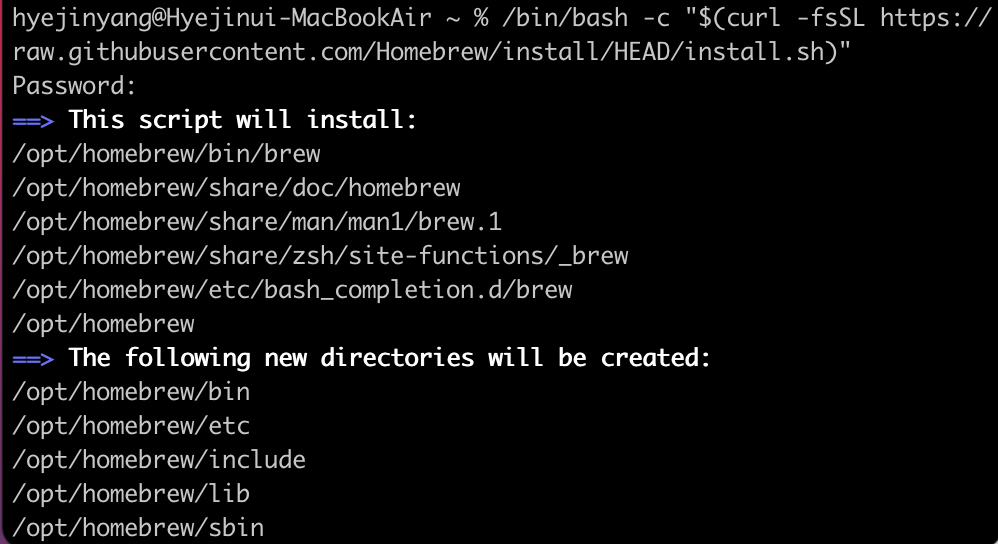
\includegraphics[width=300pt]{hw3_homebrew.png}
	\end{center}
\end{figure}

\subsection{iTerm2 설치}
맥OS에서 공식 터미널 대신 사용할 수 있는 가상 터미널 애플리케이션이다.
iTerm2는 검색 및 하이라이트, 복사, 붙여넣기 히스토리 등
기본 터미널 애플리케이션보다 다양한 기능을 제공하고 있다.

\vspace{3mm}
\noindent
설치 명령어 : 
brew cask install iterm2

\newpage

\subsection{자체 개발환경에서 작성한 hw3 파일 리스트}
\begin{figure}[!htbp]
	\begin{center}
		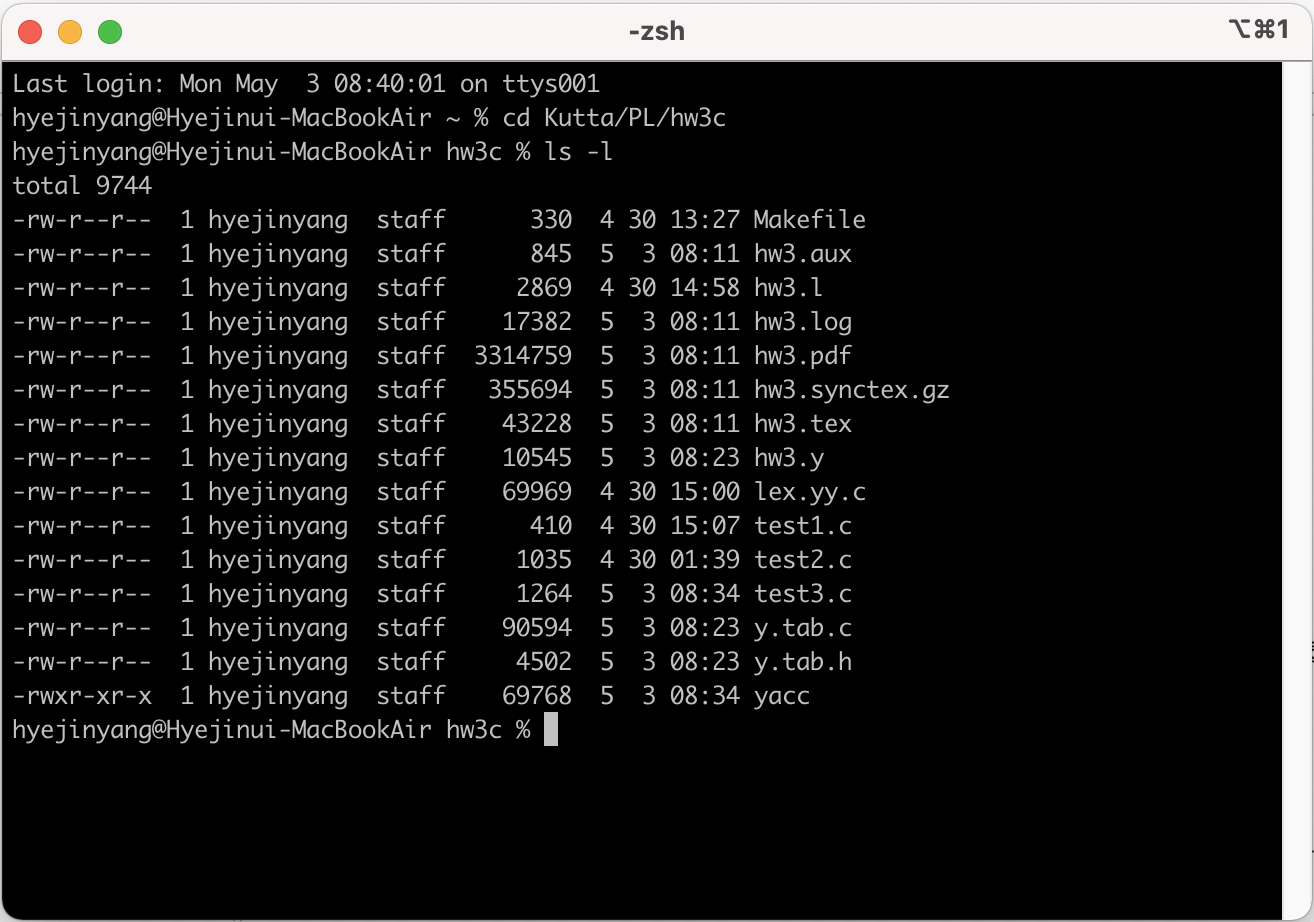
\includegraphics[width=300pt]{hw3_file_list.png}
	\end{center}
\end{figure}

\subsection{자체 개발환경에서 작성한 Makefile}
\begin{figure}[!htbp]
	\begin{center}
		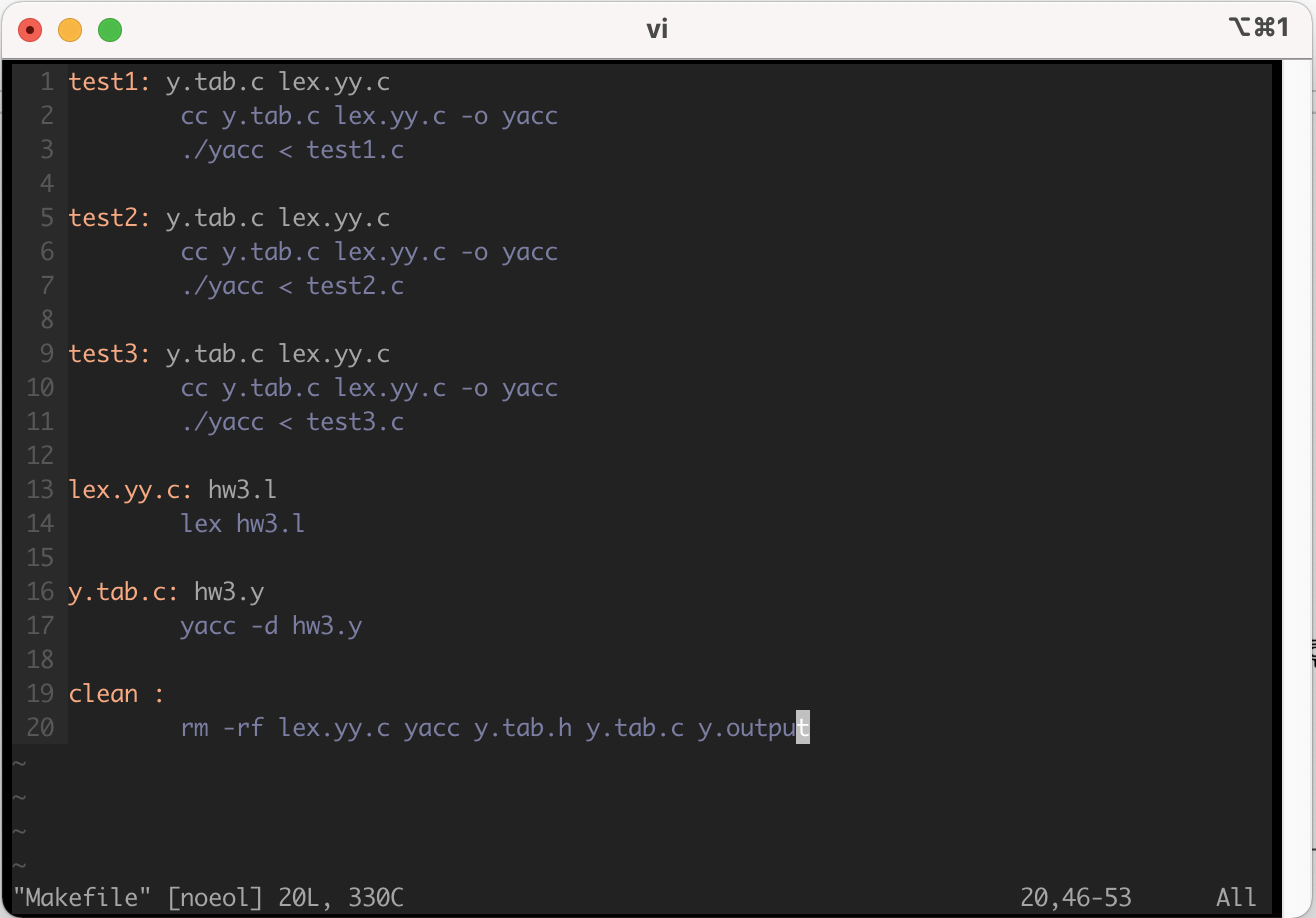
\includegraphics[width=300pt]{hw3_makefile.png}
	\end{center}
\end{figure}

\newpage

\subsection{자체 개발환경에서 테스트 진행 모습}
\begin{itemize}
	\item {test1}
	\begin{figure}[!htbp]
		\begin{center}
			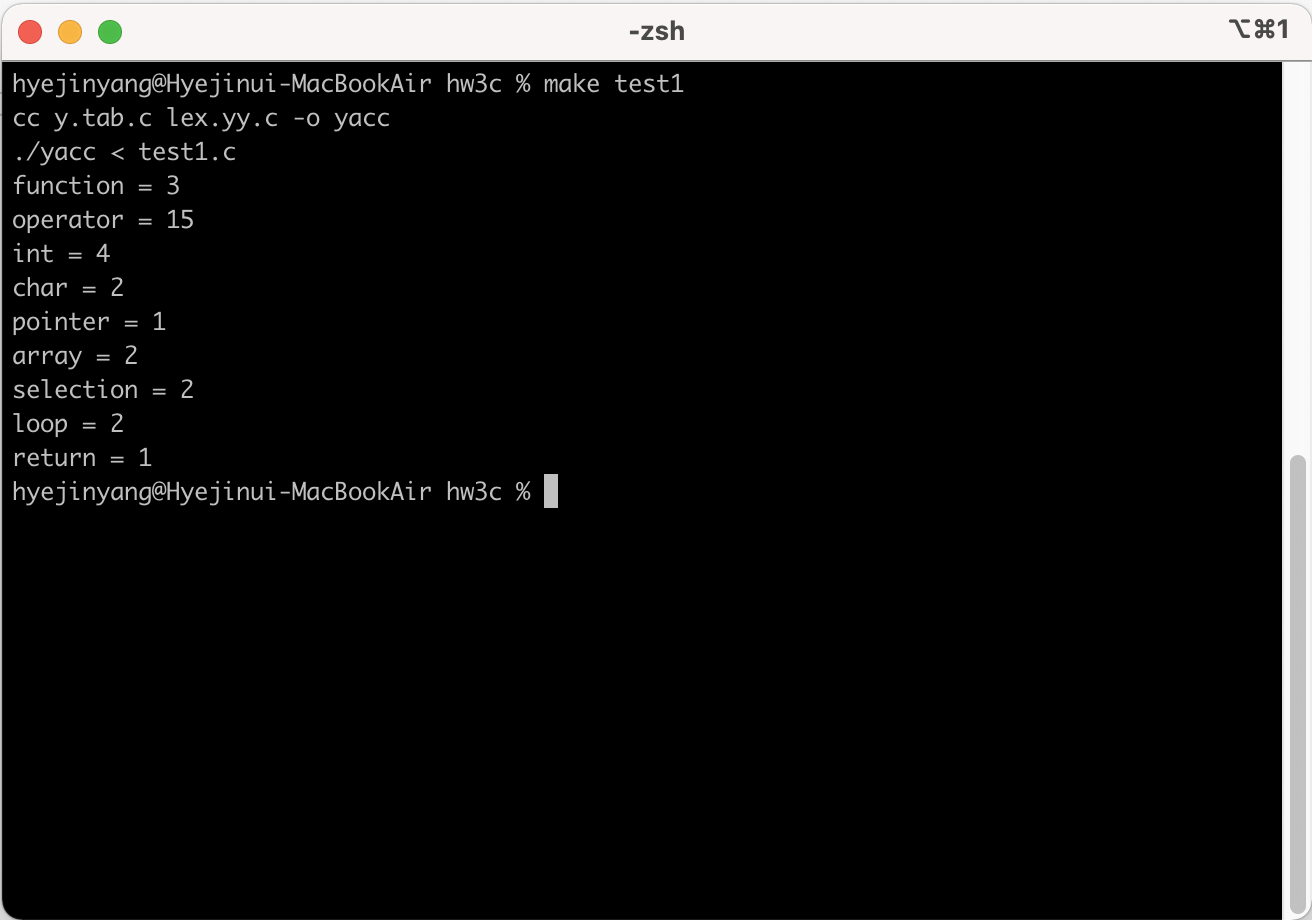
\includegraphics[width=215pt]{hw3_maketest1.png}
		\end{center}
	\end{figure}
	\item {test2}
	\begin{figure}[!htbp]
		\begin{center}
			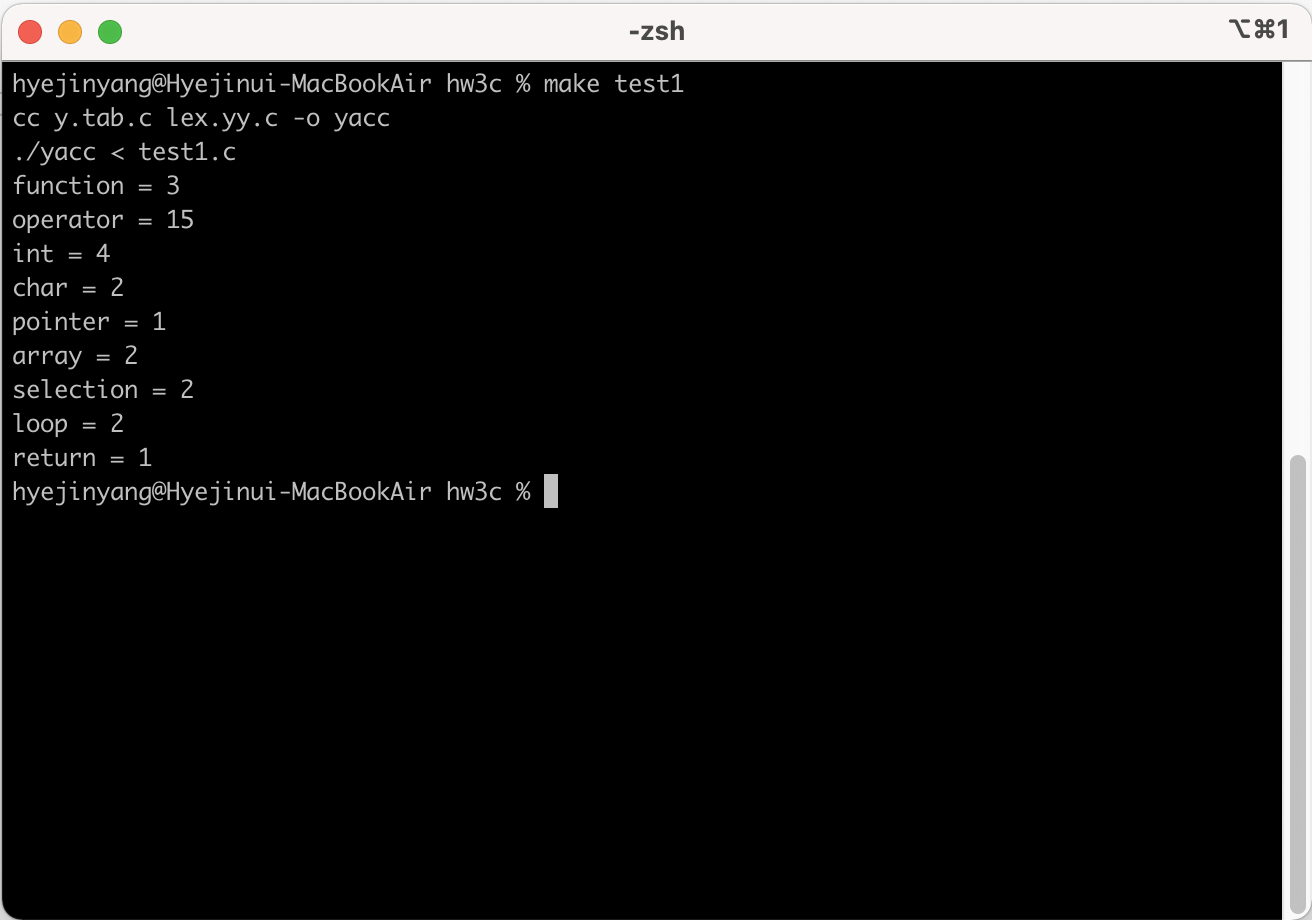
\includegraphics[width=215pt]{hw3_maketest1.png}
		\end{center}
	\end{figure}
	\item {test3}
	\begin{figure}[!htbp]
		\begin{center}
			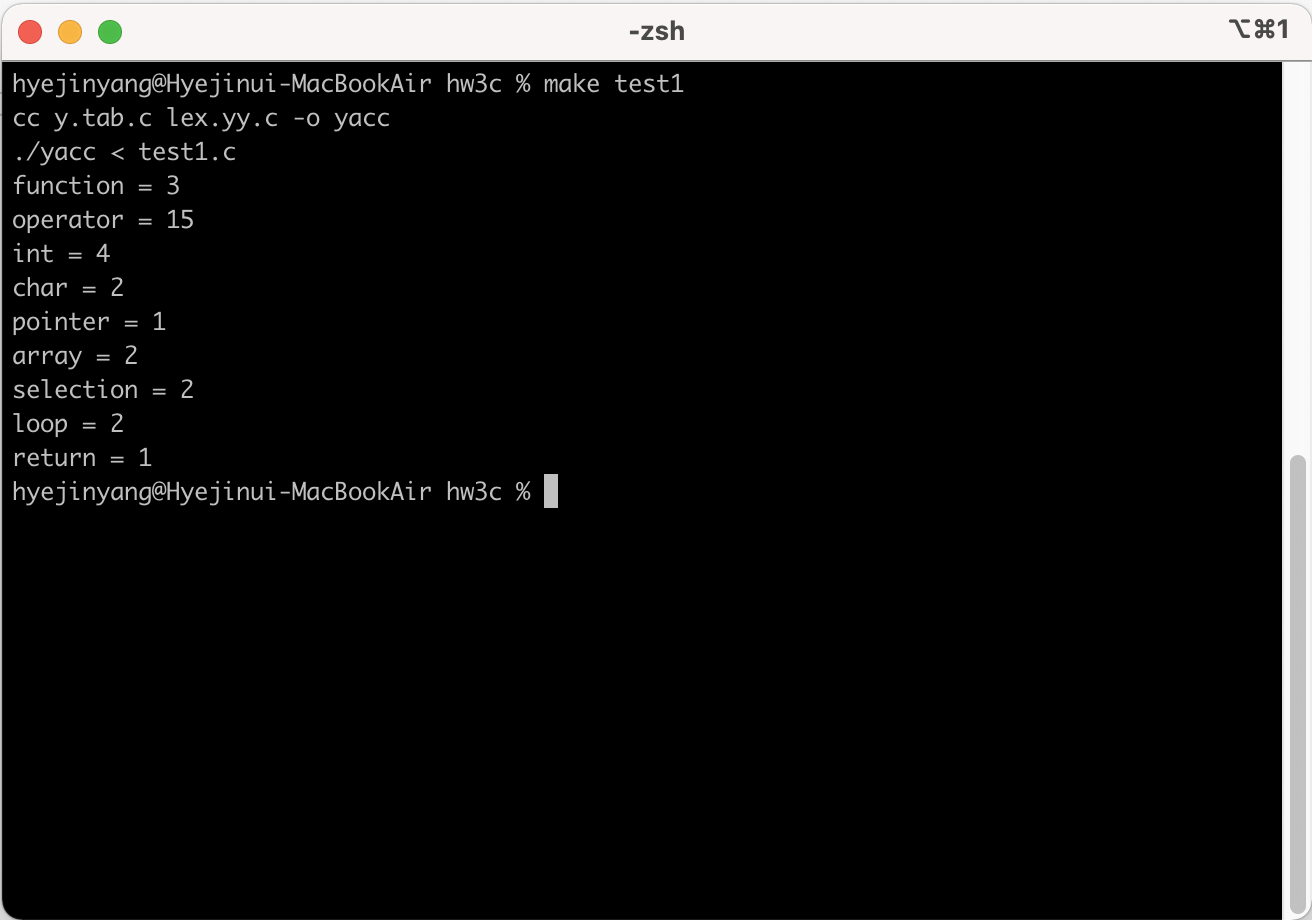
\includegraphics[width=215pt]{hw3_maketest1.png}
		\end{center}
	\end{figure}
\end{itemize}

\end{document}

%------------------------------------------------